
\section{Calculating spectra, the SPEC program}
\label{sect:spec}
\index{SPEC}
\index{Spectral analysis} 

The SPEC program is used for making spectra of many seismic signals 
in a semiautomatic manner. It can be used for several investigations: 

A: Making a large series of signal spectra, which can be corrected for instrument and path.  

Average spectra are calculated. There are two options for further processing the calculated spectra:  \newline
Option (1): Calculate acceleration density spectra which are plotted compared to the Peterson noise model.\index{Peterson noise model}\newline
Option(2): Using the slope of the flat part of the displacement spectra to calculate the near surface attenuation kappa (see \ref{subs:spec}.  \index{Kappa, determine}

B: Making relative spectra of seismic events or background noise in order to determine the soil response. When using relative spectra of horizontal versus vertical components, this is referred to as the Nakamura\index{Nakamura}\index{Soil amplification}\index{Spectral parameters}\index{Spectral ratio}\index{Quality factor, correct for}\index{Quality factor, determine by spectra} method \citep{nakamura1989}. 

C: Making relative spectra of signals from two stations in order to determine Q. The program makes output files for generating GMT plots in addition to standard SEISAN plots. 

Note: Parameter file has changed between SEISAN 7.2 and 8.0 (number of windows and overlap has been added). \newline
The program can technically operate in two ways: (1) Making relative spectra of a series of pairs of stations terminated by the average spectra, (2) Making a series of spectra for a number of stations and events. The spectra can be corrected for distance, Q, and instrument response. In addition, the spectral levels can be expressed in m\index{Moment}oment or moment magnitude calculated in the same way and with the same units as in MULPLT. All relevant parameters are taken from the CAT files, the CAL files and the input parameter file for SPEC. Window selection for the spectra can be specified to be related to the P, S arrival times or the earthquake origin time and it is thus possible to automatically make e.g. S-wave spectra of a large set of stations and events. Op\index{Noise spectrum}tionally, noise spectra, can be calculated together with the signal spectra. The noise window is selected at the start of the waveform file. \newline
Before the program is started up, the input files must be prepared. The program need two input files. The parameter file (default spec.par) gives the parameters to use and the list of stations to process. The event file (default spec.inp) is a CAT file with events to use or a \texttt{filenr.lis} type file with waveform file names (can only be used if no readings are needed, like for Nakamura studies). An example of a spec.par and spec.inp file is found in DAT. These files can be used immediately with the test data set. 

The program produces several output files. The main output is in \texttt{spec.out} with the parameters used, the station event combinations used and error messages. The other files are giving output of most graphs shown. These ASCII output files can be used in other plotting programs, however they have been specifically formatted for the SEISAN GMTXY plotting script. Note that the numerical values given for the spectral output given in those files is the same that appear on the plots and the values are linear. So if a spctrum has been instrument corrected and smoothed, that is what is given. Similarly if a relative spectrum is used.  The number of files depends on number of stations used. Examples of files could be 

\begin{tabular}{lp{10cm}}
\texttt{spec\_all\_ASK\_\_S\_\_Z.out} & All spectra from ASK, S  Z \\
\texttt{spec\_all\_BER\_\_S\_\_Z.out} & All spectra from BER, S  Z \\
\texttt{spec\_all\_gmt.out} &   All spectra from ASK and BER \\
\texttt{spec\_ave\_ASK\_\_S\_\_Z.out} & Average spectrum from ASK, S  Z \\
\texttt{spec\_ave\_BER\_\_S\_\_Z.out} & Average spectrum from BER, Z  Z\\
\end{tabular}

In order to plot these files with GMTXY (only Unix), give e.g. command

\texttt{gmtxy spec\_all\_ASK\_\_S\_\_Z.out}
\newline
There is one more output file, spec\_amp.out, which gives the log log spectra of  of all traces calculated (possibly instrument corrected) before smoothing takes place.
\index{spec\_amp.out}
\index{Spectral output file}
\newline
Limitations of amount of data: The program is set up to handle 300 spectra of up to 30000 points each for one run. The dimensions can be increased in spec.for, however the program must then be recompiled. The spectral windows are 10\% tapered. The analyzed signals will be checked for clipping and rejected if clipped. A message is then given in spec.out 

\index{Spec.par}
The \texttt{spec.par} file The file contains alternate lines of parameter names and parameter values, and must contain the number of lines shown in the example below. 

\verbatiminput{include/spec.par}

The parameters: \newline
\textbf{Selection criteria}: Determines how the start of the time window is selected. 1: Start with the P-arrival time, 2: Start with the S-arrival time, 3: Start with the S-arrival time calculated from the P-arrival time assuming a P to S velocity ratio of 1.78, 4: Start with 'start' (see next parameter) seconds after the origin time as given in the CAT file header. This option can be used if no readings are available in the CAT file. When using a P or S-time for start of window, the program uses the first P or S phase found in the CAT file for a given station. Component is of no importance here, so there is only a need for 
e.g. one P-time for the station being processed if 3 component data is used. This is also the case when rotating the signal, see below. However, on the trace plots, only readings on those components shown will be seen on the plots. 

\textbf{Start}: If the selection criterion is 1,2 or 3, this is the number of P or S travel times (from the origin) used to find start time of window. Use 1.0 if the window shall start exactly at the phase time picked. If selection criteria is 4, start is the number of seconds after the origin time. 

\textbf{Window length, \#of windows, overlap}: 

\begin{itemize}
\item[-]
Window length: Window length in secs for both signal and noise (if selected) . 
\item[-]
\# of windows: If more than 1, spectra will be made in several windows following the first window 
and average spectra will be made. This option can only be used if selection criteria is 4. Used for 
noise studies or Nakamura studies. 
\item[-]
Overlap: Windows can overlap (factor $<$ 1.0) exactly follow each other (factor=1.0) or have gaps 
(factor $>$ 1.0). E.g. 0.9 is equal to 10 \% overlap. 
\end{itemize}

\textbf{Number of times to smooth}: Number of times to smooth, 0 means no smoothing. 

\textbf{Gain factor of channel 1}: Factor that the spectral level for channel 1 is multiplied with. This can be used if the response shape is the same for the two channels and only the levels are different. If the shape is also different, set factor to 1 and use response removal \index{Response removal}below. 

\index{Noise spectrum}
\textbf{Noise spectrum}: If 0, no noise spectrum, if 1, make noise spectrum. The noise window is taken from the beginning of the trace and the window length is the same as given above. 

\textbf{Make relative spectra}: If zero, no \index{Relative spectra}relative spectra, if 1, make relative spectra. The relative spectra will appear one on each page, and the average relative spectrum on the last plot (see Figure 
\ref{fig:spec-example}
). If no relative spectra are chosen, only one trace and one spectrum is shown per page and the average spectrum is shown on the final plot. MUST BE SET to 1 to calculate Q, see below. 

\textbf{Plot pics}: If 1, the phase pics in the CAT file spec.inp will be plotted. 

\textbf{Frequency band used}: Lower and upper frequency bands for the spectral plots. 

\textbf{Response removal}: If 0, no response is removed, else 1: displacement, 2: velocity, 3: acceleration (units is nm, nm/s and nm/s*s), 4: Power spectral density in dB relative to ((1m/s**2)**2)/Hz. This option is used for seismic background noise studies.\index{Power spectral density}\index{Background noise}\index{Noise study}, 5: Determine kappa. The flat part of the spectrum (frequency below corner frequency) is approximated by a straight line and kappa calculated for each event and the average at the end (in spec.out file and on final plot). The spectrum will normally be corrected for Q, BUT NOT kappa. For more details, see \citep{havskov2010}. Make sure to set appropriate frequency limits and correct distance corrections. Can be used for both P and S-spectra. A cal file for each channel must be available in the CAL directory (see section 4.6). For relative spectra, the response removal has no importance if the response is the same for the channels compared. A simple correction can be made with "Gain factor of channel 1" parameter above. NOTE: If moment or magnitude spectrum is made, response removal MUST be 1. 

\textbf{Rotate components}: If 1, the horizontal components are rotated. This means that if the user has specified N or E, radial or transverse respectively will be used instead. The original data remain unchanged. If start time of spectra are chosen by using P or S, there must be a reading from those components if the pics are to be plotted. If the parameter is zero, no rotation is done. See also MULPLT for more details of rotation. 

\textbf{Q0, qalpha and kappa:}

Q-correction: \newline
Parameters in Q-relation Q = Q0**qalpha used for spectral correction (see also section on MULPLT for standard attenuation relations). Only used if response is removed. If first 2 parameters are 0,0, no Q-correction. New from SEISAN7.2 is that a kappa correction also can be used (see MULPLT spectral section). 

Calculation of Q: \newline
If Q0 and qalpha is set to -1,0, the relative spectra will be used to calculate q as a function of f (see standard relations in MULPLT section) and the plots will show q as a function of f. This can be used for both P-waves and S-waves. The distance correction MUST be set, S-velocity must be given (see below) and it is recommended to assume body wave spreading (amplitude proportional to 1/distance, factor is 1.0 below). If the response of the 2 stations is not identical, correction for response must also be made. There must be an origin time and phase readings for components used must be available in order to calculate Q. Q is calculated as  pi * f * (t2-t1) / (ln(A2(f)/A1(f)) + alpha * ln(t2/t2)), where A1 and A2 are spectral levels at frequency f for the two stations, t1 and t2 are travel times and alpha is geometrical spreading exponent (1.0 is body wave spreading). Q values lower than 1 and higher than 5000 are not used, the Q(f) plot might then display a long straight line. The Q=Q0*f**qalpha is calculated from the 'good' values'. 

\textbf{Distance correction alpha}: The spectral amplitudes are multiplied by R**(distance correction) if different from zero. This option MUST be set if moment or moment magnitude options (see below) are selected as well as calculation of Q. However, it can be used without instrumental correction. For body waves, use 1. Note that the geometrical spreading use here is simpler than used in MULPLT. 

\textbf{Minimum correlation coefficient and minimum signal to noise ratio for kappa}: The minimum correlation coefficient and signal to noise ratio for an event to be included in average kappa. The coefficients are from the linear fit to the flat part of the spectrum. 

\textbf{Velocity and density}: Velocity (km/sec) and density (g/cm*cm) used for calculating moment spectra. If set to 0,0, no moment spectra are calculated. See section on MULPLT for details of calculation. 

\textbf{Magnitude spectrum}: If 1, the spectral level is converted to moment magnitude, see MULPLT for details of calculation. 

\textbf{Stations and components}: Station-component pairs used, one pair per line, format (a5,1x,a4,1x,a5,1x,a4). If no relative spectrum is used, the first station-component on the line is used. 

Averaging in spec: \newline
Q: For each frequency, the average linear 1/Q and corresponding sd is calculated. The upper and lower bounds are calculated by subtracting and adding the sd. These values are then converted back to Q and finally the log is taken. Only the `good' individual values are used. There is a possibility that the lower bound becomes negative. In that case, the log Q is set to zero. Because the average is made in 1/Q, the upper and lower bounds curves will not be symmetric around the average Q-curve. 

Power spectrum: For each frequency the dB values are averaged and upper and lower curves should be symmetric. 

Kappa: Same as for Power spectrum. 

Other spectra: The linear spectra or relative spectra are averaged. The sd used in the log spectra are calculated by subtracting log average spectrum from log(average spectrum + sd). 

Running the program: \newline
The program gets the first pair of stations (or one station) from spec.par, calculates the spectra using the list of events in spec.inp and at the end of the station list, calculates the average spectral ratios for all pairs (max 100). All spectra are then shown on one plot together with averages and standard deviation. Then the next pair of stations is processed in the same way and the program continues until the end of file spec.par. Each pair of stations with signals and spectra is plotted on one page. If no relative spectra are made, the plots look similar except that only one station is shown. Hard copy plots are made for each page and sent to the printer if specified (see below). The hard copy postscript file is called \texttt{spec.eps} and when the program finishes, a file with the last plot is available on the disk. For each spectrum (relative or single), the average spectrum (or Q) is calculated both as an average of the log spectrum and as an average of the linear spectrum. There is no frequency weighting and since all values shown on the plot are used, the average value will be more representative of the high frequency part of the spectrum since there are more values. This can be regulated by choosing 
another frequency range. The average spectra shown on the last plot are log-averages. If option to calculate Q is used, the plots show 1/Q as a function of frequency instead of relative spectra (proportional to relative spectra). For each event,  Q0 and qalpha are calculated. 

When calculating kappa, the average spectrum do not have much physical meaning since the averages are made from absolute spectra of events that might have very different moments. So the kappa calculated from the average spectrum is not to be used. 

Interactive output of level and frequency: With a spectral ratio (or Q) plot on the screen, position the cursor at the point of interest on the spectrum and click. The level and frequency will now be displayed on the right side of the plot. 

The output file spec.out gives details of the run like averages and missing data. The output file spec\_ave.out gives the x and y-values of the average spectrum IF IT HAS BEEN PLOTTED ON THE SCREEN. File spec\_rel.out gives the values of the relative spectra. 

There are 4 interactive input options: 

0: All spectra are calculated but not sent to the plotter or screen except the last plot with the average spectra (sent to both screen and printer). Used for checking the files or making a final run. If no relative spectrum is chosen, no final plot is made. For each station and event combination, check lines are written out on the screen. 

1: All plots are shown on the screen, but not sent to the laser printer. 

2: All plots are shown on the screen and at the same time sent to the laser printer. 

3: No plots are shown on the screen, all are sent to the laser printer. For each station event combination, check lines are written to the screen. 

4: Only final plot on laser.

5: No plotting so no graphics window come up anytime. Can be used e.g. for batch mode.

How to run the program with only waveform files available: Two options: 

(A) Using S-files \newline
Step 1: Generate S-files in your local directory with AUTOREG, \newline
Step 2: Make the spec.inp file with COLLECT. 


(B) Using \texttt{filenr.lis} \newline
Step 1 : Make a dirf of waveform files to use \newline
Then use \texttt{filenr.lis} as input file name 



With only waveform files and no readings in the spec.inp file, it is only possible to use option 4 (absolute time) for start criteria. Since the events have not been located, the "origin time" read from the S-files will be identical to the waveform file start time, so the parameter "start" can then be set to number of seconds after waveform file start time. Figure 
\ref{fig:spec-example}
shows an example. 

\begin{figure}
\htmlimage{scale=2.0}
\centerline{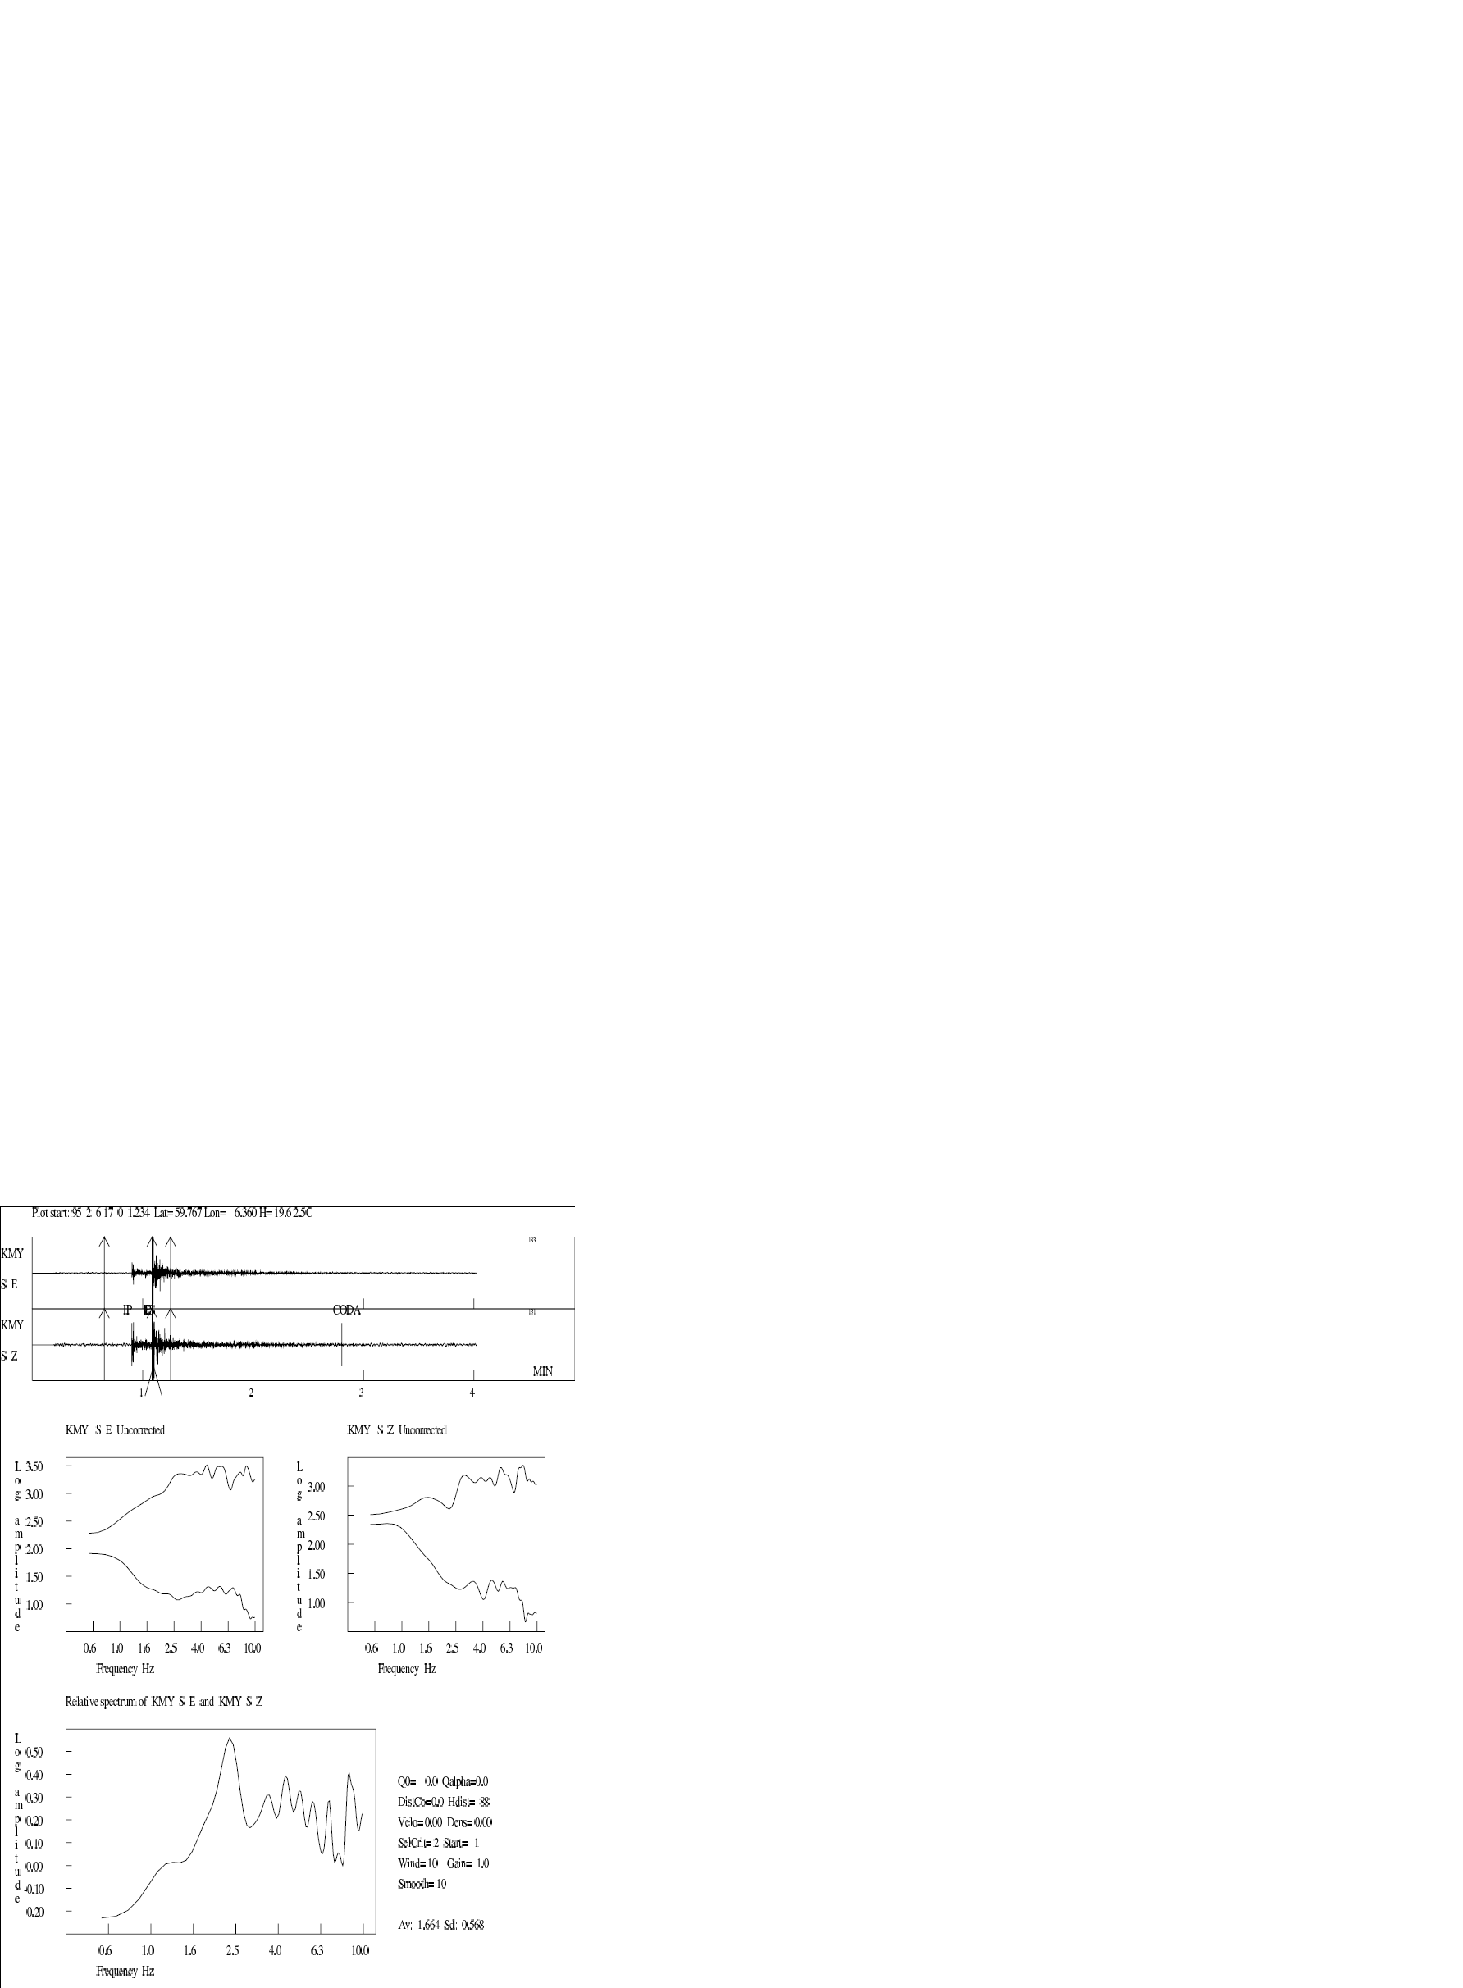
\includegraphics[width=0.9\linewidth]{fig/spec-example}}
\caption{
An example of using the SPEC program. On top the original traces are shown with windows chosen, in the middle the spectra of each channel and at the bottom, the relative spectrum. Lower right shows the input parameters used. In some cases (kappa and Q) the values calculated for this case are also shown.}
\label{fig:spec-example}
\end{figure}


\begin{figure}
\htmlimage{scale=2.0}
\centerline{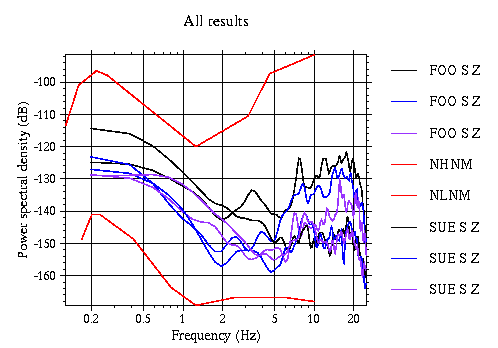
\includegraphics[width=0.9\linewidth]{fig/fig43}}
\caption{An example of a GMT plot. The figure shows an 
example of making noise spectra of several traces.}
%\label{fig:}
\end{figure}

